\documentclass{report}
\usepackage{graphicx} % Required for inserting images
\usepackage[italian]{babel}
\usepackage{tikz}
\usepackage{hyperref}
\usepackage{amsmath}
\usepackage{xcolor}
\usepackage{float}
\usepackage{soul}
\usepackage{listings} % Per evidenziare il codice

\definecolor{lightgray}{rgb}{0.9,0.9,0.9} % Definizione colore sfondo
\definecolor{darkgreen}{rgb}{0.0, 0.5, 0.0}

\lstset{
    backgroundcolor=\color{lightgray}, % Sfondo grigio
    basicstyle=\ttfamily, % Font monospaziato
    % frame=single, % Bordo attorno al codice
    tabsize=4, % Dimensione tabulazione
    breaklines=true, % Permette di andare a capo automaticamente
    numbers = left,
    numberstyle=\small\color{gray}
}

\title{\huge\textbf{{Controllo degli Accessi}}}
\date{Parte I}

\begin{document}

\maketitle

\tableofcontents
\newpage

\chapter{Introduzione}

\noindent Il \textbf{controllo degli accessi} valuta l'accesso richiesto alle risorse dagli 
utenti autenticati e, sulla base di \textit{regole di accesso} (definite all'interno)
del sistema, determina se l'accesso sia garantito o negato.

Si occupa solamente dell'\textbf{accesso diretto}. Si basa su due concetti:
\begin{itemize}
    \item \textbf{Autenticazione/Identificazione} dell'utente che fa la richiesta
    \begin{itemize}
        \item importante anche per le problematiche di \textit{accountability}; posso
        analizzare i log per capire chi ha fatto che cosa nel caso ci sia un problema
    \end{itemize}
    \item \textbf{Correttezza delle autorizzazioni} con cui l'accesso viene valutato
\end{itemize}

\section{Politiche, modelli, meccanismi}
È utile fare una distinzione tra:
\begin{itemize}
    \item \textbf{Politiche:} sono i requisiti di protezione ad alto livello che voglio applicare 
    al mio sistema 
    \item \textbf{Model:} viene usato per rappresentare la politica 
    \item \textbf{Meccanismi:} implementano la politica con \textit{hw} e \textit{sw}
\end{itemize}

\noindent Risulta utile fare questa distinzione perché comporta dei vantaggi: posso 
verificare se il modello è corretto rispetto alla politica che ho definito; lo 
stesso meccanismo può essere usato per implementare politiche o modelli diversi.

\subsection{Meccanismo}
In letteratura prende il nome di \textit{reference monitor}, deve soddisfarre le 
seguenti proprietà:
\begin{itemize}
    \item non può essere modificabile; nel caso in cui venga fatto me ne devo accorgere 
    \item non può essere bypassabile 
    \item deve essere confinato ad una specifica parte del mio sistema (non distribuito)
    \item deve essere abbastanza piccolo per essere soggetto a processi di verifica formale
\end{itemize}

\noindent Il meccanismo deve essere sicuro rispetto ai canali di comunicazione non 
legittimi:
\begin{itemize}
    \item \textbf{Storage channels:} le parti di memoria, prima di essere rese disponibili 
    ad altri dati, dovrebbero essere \textit{pulite} (se cancello un dato non è che \textit{sparisce} dalla 
    memoria fisica dal computer \dots)
    \item \textbf{Covert channels:} canali non intesi per il trasferimento di informazioni
    che possono essere usati per inferire informazioni
\end{itemize}

\subsubsection{Alcuni principi di design}
\begin{itemize}
    \item \textit{Separazione dei privilegi:} non dare troppo \textit{potere} ad un solo utente 
    \item \textit{Privilegio minimo:} voglio darti il minimo privilegio di cui hai bisogno
\end{itemize}

\section{Processo di sviluppo di un AC}
Una volta definito il modello, posso verificare due aspetti:
\begin{itemize}
    \item \textbf{Completezza:} verificare che hai rappresentato tutti i requisiti di sicurezza della politica
    \item \textbf{Consistenza:} dev essere privo di contraddizioni (un utente ha sia accesso/negazione per una risorsa)
\end{itemize}






\chapter{Discretionary (DAC) policies: approcci base}

\noindent Sono politiche basate su:
\begin{itemize}
    \item \textbf{identità} degli utenti 
    \item definizione di regole di accesso (\textbf{autorizzazioni}), che stabiliscono
    \textit{chi può fare che cosa}
\end{itemize}

\noindent Definite \textit{discrezionale} perché gli utenti che sono proprietari 
dei dati possono amministrarli come vogliono, \textit{a loro discrezione}; tipicamente, 
non ho un unico amminstratore, ma ci sono più amministratori proprietari delle risorse: è 
in mano a qualcuno stabilire chi può accedere o meno alle risorse (non è escluso avere 
un unico amministratore).

\section{Un esempio di modello}
Si usa la \textit{matrice degli accessi}, è una rappresentazione astratta della 
politica di protezione del sistema.

\noindent Formalmente, è caratterizzato da una tripla $(S, O, A)$ che rappresenta 
lo stato del sistema, dove:
\begin{itemize}
    \item $S$ è il set degli utenti 
    \item $O$ è il set delle risorse, dove $S \subset O$ (un soggetto può essere anche un processo, e può 
    essere anche una risorsa \dots)
    \item $A$ è la matrice, dove:
    \begin{itemize}
        \item le righe corrispondono ai soggetti 
        \item le colonne corrispondono agli oggetti 
        \item $A[s, o]$ riporta i privilegi di $s$ su $o$
    \end{itemize}
\end{itemize}

\begin{figure}[H]
    \centering
    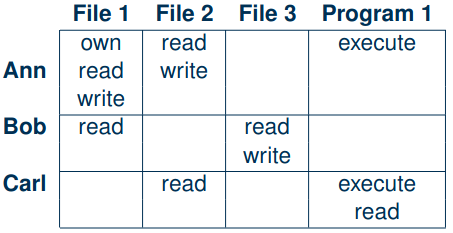
\includegraphics[width=0.6\linewidth]{images/dac1.png}
\end{figure}

\noindent I cambi di stato del sistema vengono fatti con dei comandi che chiamano delle \textbf{operazioni primitive}:
\begin{itemize}
    \item \texttt{enter} $r$ into $A[s,o]$
    \item \texttt{delete} $r$ from $A[s,o]$
    \item \texttt{create} subject $s$
    \item \dots
\end{itemize}

\noindent Sono della forma:

\begin{figure}[H]
    \centering
    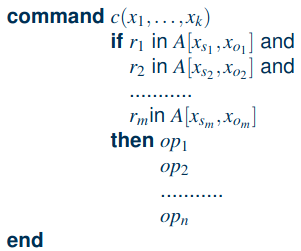
\includegraphics[width=0.45\linewidth]{images/dac-comm.png}
\end{figure}

\noindent Un esempio:

\begin{figure}[H]
    \centering
    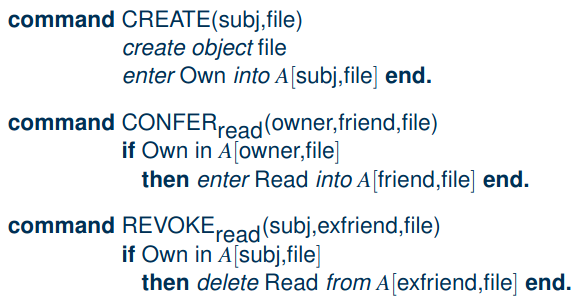
\includegraphics[width=0.65\linewidth]{images/dac2.png}
\end{figure}

\section{Trasferimento dei privilegi}
Il proprietario dei dati può dare il privilegio anche ad altri utenti.
Può rappresentato in modo formale in due modi differenti:
\begin{itemize}
    \item \textbf{Copy flag (*):} il soggetto trasferisce il privilegio ad altri; mantiene il privilegio
    \begin{figure}[H]
        \centering
        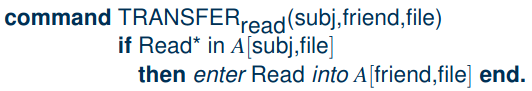
\includegraphics[width=0.6\linewidth]{images/transfer1.png}
    \end{figure}
    \item \textbf{Transfer-only flag(+):} il soggetto trasferisce ad altri il privilegio ma perde l'autorizzazione
    \begin{figure}[H]
        \centering
        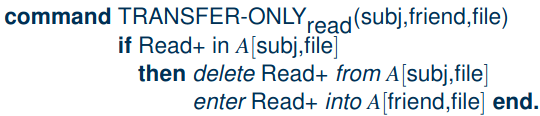
\includegraphics[width=0.6\linewidth]{images/transfer2.png}
    \end{figure}
\end{itemize}

\noindent Partendo da uno stato \textit{sicuro}, non deve accadere che applicando una o più operazioni 
si finisca in uno stato non sicuro.

\section{Implementazione della matrice}
La matrice è spesso sparsa, salvarla sarebbe uno spreco di memoria. Ci sono diversi 
approcci alternativi:
\begin{itemize}
    \item \textbf{Tabella di autorizzazione}; tabella di tuple $(S, O, A)$ non nulle
    \begin{figure}[H]
        \centering
        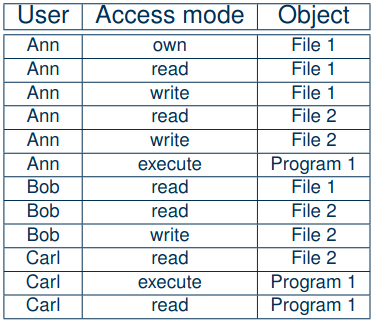
\includegraphics[width=0.5\linewidth]{images/auth-table.png}
    \end{figure}
    \newpage
    \item \textbf{Access Control Lists (ACLs)}: store by column; ad ogni risorsa associo una lista 
    che mi dice gli utenti quali operazioni possono fare
    \begin{figure}[H]
        \centering
        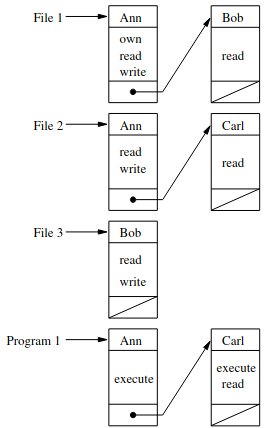
\includegraphics[width=0.4\linewidth]{images/acl.png}
    \end{figure}
    \item \textit{Capability lists}; store by row; sono come le precedenti ma vengono fatti storando per utenti
    invece che per risorse. Sono state soppraffatte dalle ACLs
    \begin{figure}[H]
        \centering
        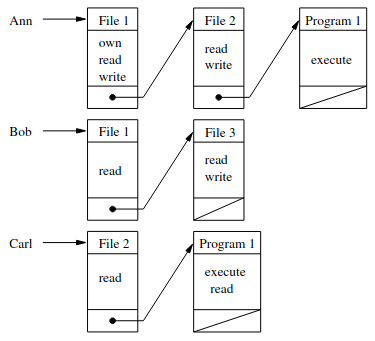
\includegraphics[width=0.5\linewidth]{images/capability.png}
    \end{figure}
\end{itemize}

\subsubsection{ACLs vs Capability lists}
\begin{itemize}
    \item non richiedono 
    autenticazione del soggetto, ma richiedono la possibilità di verificare che non siano state impropriamente 
    modificate \dots difficile da verificare (per questo non hanno avuto grande successo)
    \item le ACLs funzionano meglio quando fare delle operazioni di revoca per oggetto (ovviamente viceversa se devo fare revoche per soggetto)
\end{itemize}

\section{Debolezze di DAC}
Consentono il controllo solo sull'accesso \textbf{diretto}. Sono vulnerabili ai \textit{trojan 
horses}, ovvero accessi indiretti.

\begin{figure}[H]
    \centering
    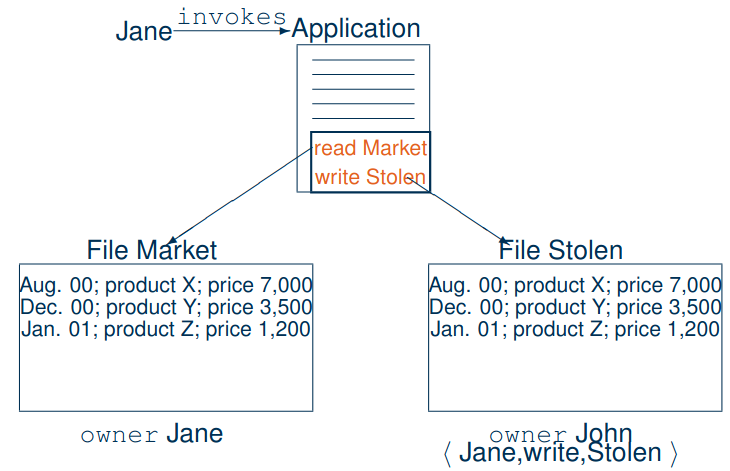
\includegraphics[width=0.8\linewidth]{images/trojan.png}
\end{figure}

\noindent L'idea è che vengono lasciate delle \textit{operazioni nascoste} in una applicazione per 
poter fare delle operazioni che normalmente non si avrebbe l'autorizzazioni di fare.

$\rightarrow$ è un accesso indiretto; è il processo che Jane sta eseguendo a chiedere l'accesso ai file



\chapter{Mandatory (MAC) policies}
\noindent Partono dall'assunzione che c'è una differenza tra \textit{utente} e \textit{soggetto}; è ciò 
che serve per bloccare i \textit{trojan horses}:
\begin{itemize}
    \item \textbf{Utente:} essere umano (di cui mi fido)
    \item \textbf{Soggetto:} processo nel sistema; opera per conto dell'utente; \textbf{non sono fidati} 
\end{itemize}

\noindent La politica più comune sono quelle \textbf{multilivello}: ogni soggetto e 
oggetto sono classificate con una etichetta. Si differenziano in politiche che si focalizzano su:
\begin{itemize}
    \item confidenzialità (Bell La Padula)
\end{itemize}

\textit{oppure}

\begin{itemize}
    \item integrità (Biba)
\end{itemize}

\section{Classificazione di sicurezza}
Ogni soggetto ed oggetto è associato ad una coppia di elementi:
\begin{itemize}
    \item \textbf{Livello di sicurezza:} livelli su cui è definita una relazione d'ordine totale (li posso mettere \textit{in fila}).
    \begin{center}
        $Secret > Confidential > Unclassified$
    \end{center}
    \item \textbf{Categoria:} insieme di elementi su cui non è definita alcuna relazione di ordinamento; serve 
    per partizionare aree differenti del sistema. Ad esempio, l'università ha un sacco di informazioni di vario 
    tipo: anagrafiche, finanziare, accademiche, \dots. 
    
    \noindent Hanno l'obiettivo di classificarle in classi diverse. Viene fatta 
    sia lato oggetto che lato soggetto.
\end{itemize}

\noindent La combinazione di queste due permette di definire una \textbf{relazione di dominanza:}
\begin{center}
    $(L_1, C_1) \geq (L_2, C_2) \Leftrightarrow L_1 \geq L_2 \land C_1 \supseteq C_2$
\end{center}

Questa relazione soddisfa una serie di proprietà che, in matematica, permette di formare 
un \textit{reticolo} (quando combinata fra tutte le classi); nel nostro caso parliamo 
di \textbf{reticolo di classificazione}.

\begin{figure}[H]
    \centering
    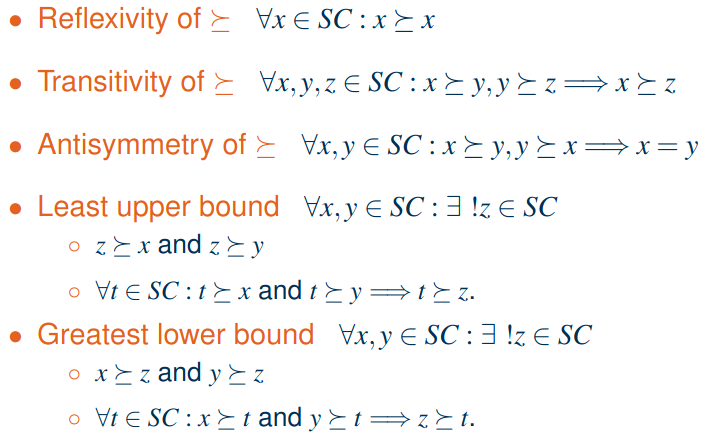
\includegraphics[width=0.8\linewidth]{images/props.png}
\end{figure}

\noindent Esempio di reticolo di classificazione:
\begin{figure}[H]
    \centering
    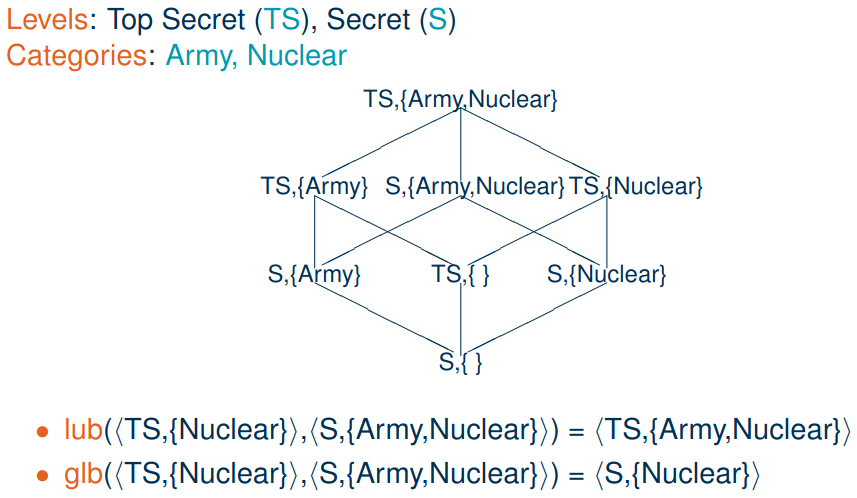
\includegraphics[width=0.8\linewidth]{images/reticolo.png}
\end{figure}

\newpage
\section{Semantica della classificazione di sicurezza}
\begin{itemize}
    \item \textbf{Classi di sicurezza}
    \begin{itemize}
        \item associato ad un \textit{soggetto}, rilfette la fiducia verso quell'utente; quanto mi fido di quell'utente 
        \item associato ad un \textit{oggetto}, riflette la sensisibilità dell'informazione
    \end{itemize}
    \item Le \textbf{categorie} definiscono l'area di competenza di utenti e dati.
\end{itemize}

\section{Bell La Padula}
È un modello che si preoccupa della confidenzialità (e non del resto).

\noindent Considerando di essere in un ambiente multilivello, l'\textbf{obiettivo} è 
prevenire flussi di informazioni ai livelli più bassi o a classi incomparabili.

\begin{itemize}
    \item \textbf{\textit{Simple property:}} un soggetto $s$ può leggere un oggetto 
    $o$ solo se $\lambda(s) \geq \lambda(o)$
    \item \textbf{\textit{*-property:}} un soggetto $s$ può scrivere un oggetto $o$ solo 
    se $\lambda(o) \geq \lambda(s)$
\end{itemize}

$\Rightarrow$ \textbf{NO READ UP}

$\Rightarrow$ \textbf{NO WRITE DOWN}

\noindent \textit{Se sono Secret, e scrivo un file secret in uno Top-Secret, non è mica un problema 
per la confidenzialità. Potrebbe esserlo se scrivo secret in un file Unclassified (potrebbe causare problemi a livelli di integrità, ma ci stiamo occupando solo di confidenzialità).}

\subsection{Proprietà di sicurezza}
Un sistema viene formalizzato come \textit{stato}
e \textit{transizioni di stato}. 

\noindent Uno stato $v \in V$ è una tripla $(b, M, \lambda)$, dove:
\begin{itemize}
    \item $b$ è l'insieme di triple $(S \times O \times A)$, ovvero l'insieme degli accessi (\textit{soggetto, oggetto, accesso})
    \item $M$ è la matrice di accesso (per rappresentare una politica discrezionale)
    \item $\lambda$ è una funzione che ritorna la classe di sicurezza associata a soggetti e oggetti
\end{itemize}

\noindent Da questa definizione segue che uno stato $(b, M, \lambda)$ è sicuro se rispetta:
\begin{itemize}
    \item \textbf{Simple security:} $\forall (s,o,a) \in b, a = read \Rightarrow \lambda(s) \geq \lambda(o)$
    
    \textit{se la tripla appartiene a b, è perché vale la simple property (classe del soggetto domina quella dell'oggetto)}
    \item \textbf{* property:} $\forall (s,o,a) \in b, a = write \Rightarrow \lambda(o) \geq \lambda(s)$
    
    \textit{se la tripla appartiene a b, è perché vale la * property (classe del oggetto domina quella del soggetto)}
\end{itemize}

\noindent Dato che un sistema può variare nel tempo, occorre formalizzare anche questo aspetto.
Viene definita una \textbf{funzione di transizione di stato} $T: V \times R \rightarrow V$, che 
trasforma lo stato in un altro che soddisfa le due proprietà.

\subsubsection{Sistema sicuro}

Un sistema $(v_0, R, T)$ è sicuro se ogni stato raggiungibile da $v_0$ con una sequenza finita di 
passi da $R$ è sicuro. Formalmente, un sistema è sicuro se:
\begin{itemize}
    \item $v_0$ è sicuro 
    \item $T$ è tale che $\forall v$ raggiungibile da $v_0$ eseguendo una o più richieste 
    da $R$, allora deve valere che:
    \begin{figure}[H]
        \centering
        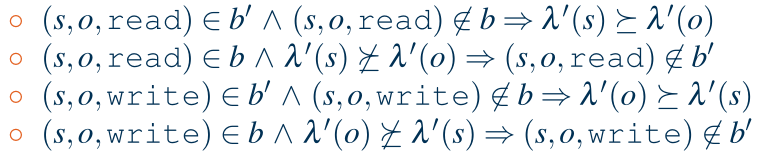
\includegraphics[width=0.8\linewidth]{images/blp-ss.png}
    \end{figure}
\end{itemize}

\subsection{\textit{BLP + tranquility}}

L'idea è di controllare ciò che fa $T$, dato che potrebbe dar vita 
a problemi di sicurezza.

\noindent Viene introdotta la \textit{\textbf{tranquility property}}, secondo cui 
il livello di sicurezza associato a soggetti e oggetti non può cambiare.

\noindent Tuttavia, questa restrizione è troppo forte da poter applicare in casi reali;
vengono così introdotti alcuni casi in cui viene \textit{attenuata}:
\begin{itemize}
    \item non tutti i cambi di livello rilasciano informazioni (cambiare verso l'alto può essere ok)
    \item soggetti fidati possono fare downgrade
\end{itemize}


\subsubsection{Altre eccezioni}
\noindent Altre eccezzioni non catturate dal modello, che richiedono di attenuare 
le restrizioni:
\begin{itemize}
    \item \textbf{Data association:} un set di valori associati potrebbe essere classificato 
    \textit{più alto} rispetto ai valori presi singolarmente 
    \item \textbf{Aggregation:} l'aggregazione di tutte le istanze diventa sensibili (ad esempio,
    la posizione di navi da guerra)
    \item \textbf{Sanitizzazione e downgrading:} dopo un certo tempo alcuni dati potrebbero 
    subire un downgrade
\end{itemize}


\subsection{Coesistenza di DAC e MAC}
Il modello BLP permette la coesistenza di DAC e MAC: oltre alle classi e 
alla relazione di dominanza, viene controllata anche la matrice di accesso.
\begin{center}
    DAC property: $b \subseteq \{(s,o,a) | a \in M[s,o]\}$
\end{center}

\noindent Se sono applicati sia DAC che MAC, solo gli accessi che li soddisfano entrambi 
sono garantiti.

\subsection{Limitazioni delle politiche mandatorie}
Le politiche mandatorie sono vulnerabili ai \textbf{canali nascosti}; sono 
canali normalmente non usati per la comunicazione, ma che possono essere usati per 
comunicare in modo illegittimo delle informazioni.

\noindent \textbf{Ogni risorsa del sistema condivisa tra processi di livelli diversi 
può essere usata per creare un canale nascosto}. I canali nascosto possono essere di tipo:
\begin{itemize}
    \item \textbf{Storage:} ad esempio un soggetto top-secret crea un file se vuole comunicare 
    qualcosa, altrimenti no; un soggetto secret prova a scrivere tale file: dall'esistenza o meno 
    deduce l'informazione 
    \item \textbf{Timing:} viene sfruttata la diversa reazione che il sistema può avere in 
    termini di tempo di risposta. 
    
    \noindent Ad esempio, blocco una stampante così che l'utente al livello più basso,
    vedendo il tempo di risposta diverso, capisce che l'altro utente vuole comunicare qualcosa
\end{itemize}

\section{Politche mandatorie per l'integrità}
L'altra proprietà da proteggere (oltre alla confidenzialità) è l'integrità. In 
maniera simile a quanto visto precedentemente, vengono definite:
\begin{itemize}
    \item \textbf{Classi di integrità:}
    di integrità:
    \begin{itemize}
        \item associate agli \textit{utenti} riflettono la fiducia che non modifichi
        informazioni in modo improprio (prima era che non vada a diffondere informazioni sensibili)
        \item associate agli \textit{oggetti} riflettono il grado di fiducia che ho dell'informazione 
        contenuta nell'oggetto e il danno potenziale che modifiche a tale oggetto potrebbero causare
    \end{itemize}
    \item \textbf{Categorie:} defininoscono l'area di competenza di soggetti e oggetti 
\end{itemize}

\section{Modello Biba}
È simmetrico a BLP:
\begin{itemize}
    \item in BLP, non posso leggere verso l'alto e non posso scrivere verso il basso 
    perché non mi fido dei processi (\textit{chi mi dice che un processo non legge informazioni 
    TS e le scrive in oggetti S?})
    \item in Biba, i soggetti non possono scrivere a livelli più alti, altrimenti comprometterebbero 
    l'integrità; non posso leggere a livello più basso perché potrei avere informazioni non affidabili
\end{itemize}

$\rightarrow$ vengono fatti ragionamenti opposti perché si hanno obiettivi diversi da raggiungere

\noindent La politica di integrità prevede:
\begin{itemize}
    \item \textbf{Simple property:} un soggetto $s$ può leggere un oggetto $o$ solo 
    se $\lambda(o) \geq \lambda(s)$
    \item \textbf{*-property:} un soggetto $s$ può scrivere un oggetto $o$ solo se $\lambda(s) \geq \lambda(o)$
    
    \textit{NB: viene segnalato al sistema ma non bloccato}
\end{itemize}

$\Rightarrow$ \textbf{NO READ DOWN}

$\Rightarrow$ \textbf{NO WRITE UP}

\subsection{Politiche alternative}
Due varianti per rilassare le restrizioni:
\begin{itemize}
    \item \textbf{\textit{Rilassare l'operazione lettura:}}
    
    \noindent Un soggetto $s$ può leggere quasiasi oggetto $o$. Dopo l'accesso, 
    $\lambda(s):= glb(\lambda(s), \lambda(o))$.
    \begin{itemize}
        \item \textit{se leggo un informazione a livello più basso, anche le mie azioni 
        si basano su informazioni meno affidabili; per questo viene abbassato il livello di integrità
        al soggetto (nel caso in cui $\lambda(o) < \lambda(s)$)}
        \item \textit{Drawback:} l'ordine delle operazioni influenza i privilegi del soggetto
    \end{itemize}
    \item \textbf{\textit{Rilassare l'operazione di scrittura:}}

    \noindent Un soggetto $s$ può scrivere qualsiasi oggetto $o$. Dopo l'accesso, 
    $\lambda(o):= glb(\lambda(s), \lambda(o))$
    \begin{itemize}
        \item \textit{posso cambiare informazioni affidabili con altre meno affidabili; per questo 
        devo cambiare la classe di integrità dell'oggetto}
        \item \textit{Drawback:} non blocca questo tipo di scritture ma si limita a segnararle
    \end{itemize}
\end{itemize}

\subsection{Limitazioni di Biba}
Il vero problema di Biba è che guarda solo un aspetto limitato dell'integrità 
delle informazioni; non basta per proteggere l'integrità.

\newpage
\section{Applicazione di BLP nelle basi di dati}

È prima di tutto necessario decidere il livello di granularità a cui associare 
le classi di sicurezza per applicare la politica mandatoria:
\begin{itemize}
    \item relazione 
    \item attributo 
    \item tupla 
    \item elemento
\end{itemize}

\subsection{Modello relazionale classico}
Ogni relazione è caratterizzata da:
\begin{itemize}
    \item \textbf{Schema} della relazione $R(A_1, \dots, A_n)$, indipendente dallo stato 
    \item \textbf{Istanza} della relazione, dipendente dallo stato, composta 
    \\ da tuple $(a_1, \dots, a_n)$
\end{itemize}

\begin{figure}[H]
    \centering
    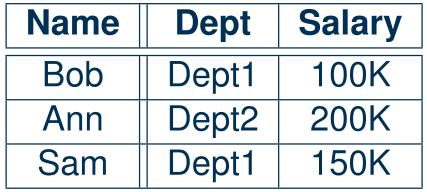
\includegraphics[width=0.5\linewidth]{images/classic.png}
\end{figure}

\noindent Gli \textbf{attributi chiave} identificano univocamente le tuple:
\begin{itemize}
    \item due tuple non possono avere la stessa chiave 
    \item le chiavi non possono avere valore \texttt{null}
\end{itemize}

\subsection{Multilevel DBMSs}
Ogni relazione è caratterizzata da:
\begin{itemize}
    \item \textbf{Schema} delle relazione $R(A_1,C_1,\dots,A_n,C_n)$, indipendente
    dallo stato 
    \begin{itemize}
        \item $C_i$, con $i = 1, \dots, n$, è il range delle classificazioni di sicurezza
    \end{itemize}

    $\rightarrow$ vengono aggiunti altri $n$ attributi per tenere traccia delle classificazioni
    \item \textbf{Set di instanze} della relazione $R_c$, dipendente dallo stato; una istanza 
    per ogni classe $c$. Ciascuna istanza è composta da tuple $(a_1,c_1,\dots,a_n,c_n)$

    \noindent L'istanza a livello $c$ contiene solo gli elementi la cui classificazione è 
    dominata da $c$
\end{itemize}

\subsubsection{Controllo degli accessi}
Il controllo degli accessi viene fatto applicando il modello BLP:
\begin{itemize}
    \item \textit{no read up}
    \item \textit{no write down further restricted} 
    
    $\rightarrow$ ogni soggetto può scrivere solo al \textbf{suo} livello
\end{itemize}

\begin{figure}[H]
    \centering
    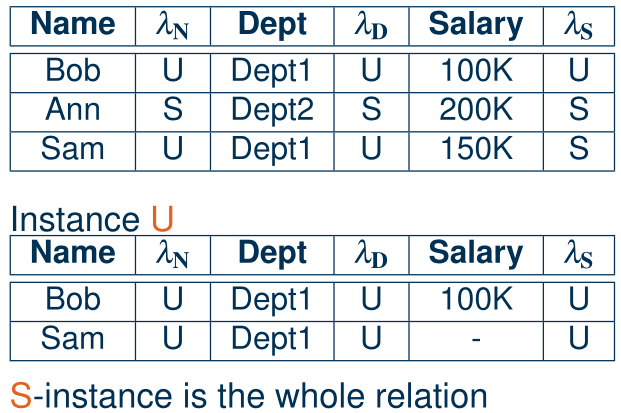
\includegraphics[width=0.7\linewidth]{images/multi-dbms.png}
\end{figure}

\subsubsection{Modello relazionale multilivello}
Per ogni tupla in una relazione multilivello:
\begin{itemize}
    \item gli attributi chiave devono avere la \textbf{stessa classe}, altrimenti 
    potrebbero avere valore nullo (riesco ad inferire qualcosa)
    \item gli \textbf{attributi non chiave devono dominare gli attributi chiave}, 
    altrimenti potrei vedere un attributo senza l'identificatore
\end{itemize}

\section{Polinstanziazione}
La polinstanziazione consiste nella \textbf{presenza di oggetti con lo stesso nome 
ma classifiazione diversa}; ovvero, tuple diverse con la stessa chiave ma:
\begin{itemize}
    \item diversa classificazione per la chiave (\textit{polyinstantiated tuples})
    \item valori e classificazione diversi per uno o più attributi (\textit{polyinstantiated elements})
\end{itemize}

\noindent Il sistema si occuperà di fare il \textit{merge} tra le varie tuple con classificazione 
diversa, restituendo sempre una sola tupla.


\subsection{Polinstanziazione invisibile}
Un soggetto a \textit{livello basso} inserisce dati in un campo che contiene già valori 
a livello più alto; il soggetto non vede i dati già esistenti.


\subsubsection{Esempio - Tuple polinstanziate}
\begin{figure}[H]
    \centering
    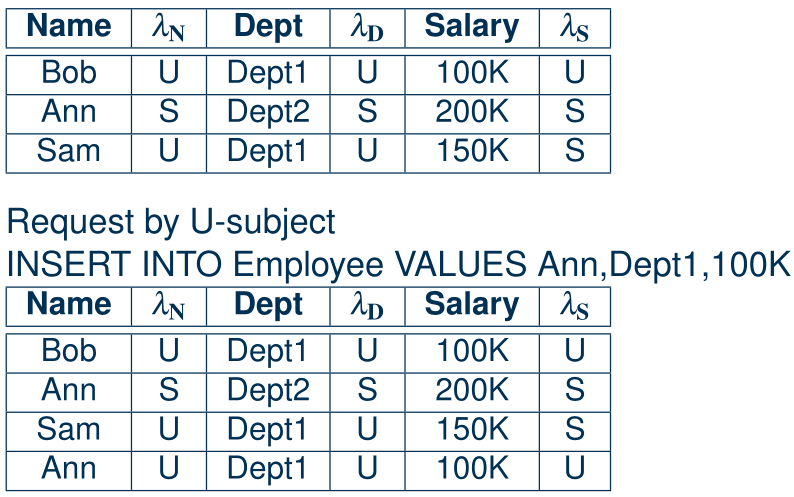
\includegraphics[width=0.8\linewidth]{images/poly1.png}
\end{figure}

\begin{itemize}
    \item Un utente U vuole inserire una tupla per Ann, dato che quella già esistente non la vede 
    \item L'inserimento di questa tupla viene permesso, dunque mi ritrovo con due tuple con lo \textbf{stesso 
    valore per l'attributo chiave} (Ann), ma con \textbf{classificazione diversa}
    \begin{itemize}
        \item non può essere impedito, perché altrimenti inferisci che Ann c'è ma non la vedi (\textbf{\textit{information leakage}})
        \item non può essere modificata la tupla già esistente (\textit{\textbf{loss of integrity}})
    \end{itemize}
\end{itemize}

\subsubsection{Esempio - Elementi polinstanziati}

\begin{figure}[H]
    \centering
    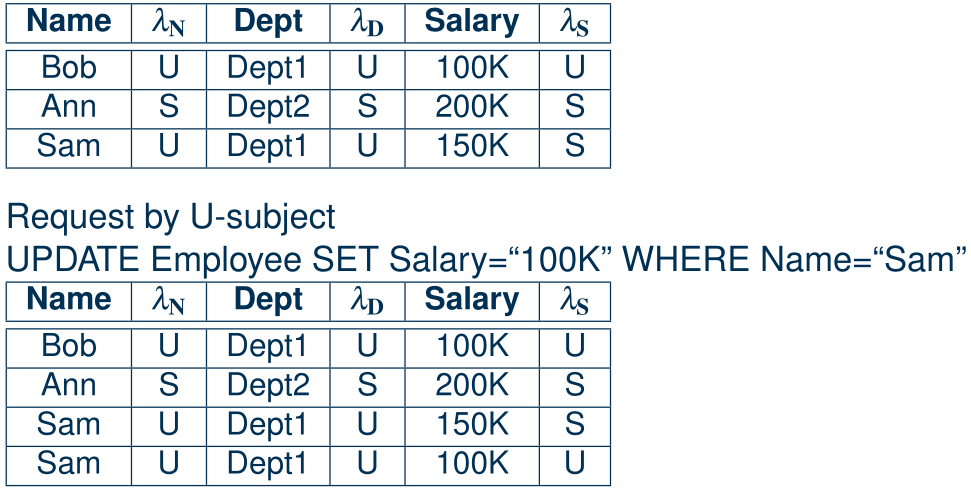
\includegraphics[width=0.8\linewidth]{images/poly2.png}
\end{figure}

\begin{itemize}
    \item Un utente U vuole fare update del salario di Sam (dato che non lo può vedere)
    \item Viene fatta un'altra tupla, dunque mi ritrovo con due tuple con \textbf{gli stessi valori per 
    l'attributo chiave, ma valori diversi per attributi non chiave}
    \begin{itemize}
        \item l'operazione non può essere impedita (\textit{\textbf{information leakage}})
        \item viene creata un'altra tupla perché la modifica viene fatta con una classe minore, 
        quindi la nuova informazione è meno affidabile di quello che ho già (\textit{\textbf{loss of integrity}})
    \end{itemize}
    
\end{itemize}

\subsection{Polinstanziazione visibile}
Un soggetto ad \textit{livello alto} inserisce dati in un campo che contiene già valori 
a livello più basso; il soggetto vede i dati già esistenti.

\subsubsection{Esempio - Tuple polinstanziate}

\begin{figure}[H]
    \centering
    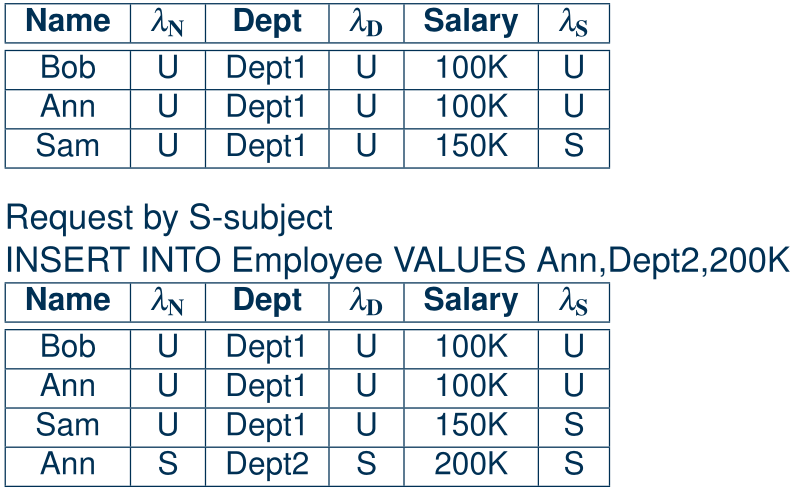
\includegraphics[width=0.8\linewidth]{images/poly3.png}
\end{figure}

\begin{itemize}
    \item Un utente S vuole modificare una tupla U 
    \item Viene creata una nuova tupla, così che la tupla U non viene toccata (senza 
    quindi creare un canale di inferenza) e salvando la nuova informazione
    \begin{itemize}
        \item L'operazione non può essere impedita, dato l'informazione S è più affidabile di quella U (\textit{\textbf{denial of service}})
        \item La tupla esistente non può essere direttamente modificata, altrimenti gli utenti U smetterebbero di 
        vederla e potrebbero inferire informazioni (dato che nell'update si andrebbe a cambiare anche la classe 
        di classifiazione d a U a S) (\textit{\textbf{information leakage}})
    \end{itemize}
\end{itemize}


\subsubsection{Esempio - Elementi polinstanziati}

\begin{figure}[H]
    \centering
    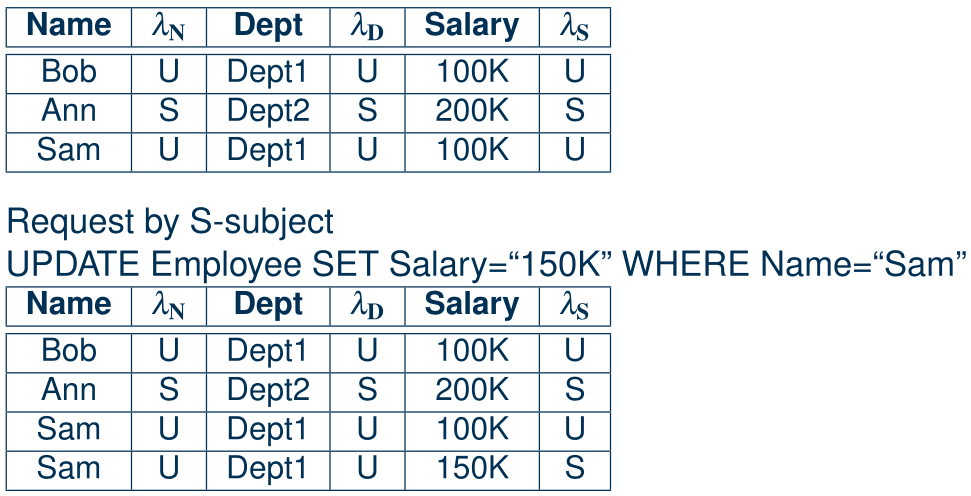
\includegraphics[width=0.8\linewidth]{images/poly4.png}
\end{figure}

\begin{itemize}
    \item Un utente S vuole modificare il salario di Sam che è U 
    \item Viene fatta una nuova tupla, dove cambia il \textbf{valore e la classe di classificazione}, da 
    U a S 
    \begin{itemize}
        \item come prima, non posso bloccare la richiesta (\textit{\textbf{denial of service}})
        \item come prima, non posso modificare direttamente la tupla esistente (\textit{\textbf{information leakage}})
    \end{itemize}
\end{itemize}

\subsubsection{Esempio di domanda all'esame}
\textcolor{red}{Parlami della polinstanziazione.} 

\noindent La polinstanziazione può essere a livello di tupla o di elemento, ed ognuna di queste 
può essere visibile o non visibile\dots

\subsection{Considerazioni}
La polinstanziazione viene fatta perché è l'unico modo per fare ciò che viene richiesto 
senza creare inferenza. 

\noindent Tuttavia, è necessario usarla perché si è cercato di applicare la politica ad un 
livello di granularità molto fine (elemento):
\begin{itemize}
    \item ho il vantaggio di avere più controllo 
    \item ho lo svantaggio di dover ricorrere alla polinstanziazione
\end{itemize}

\noindent Tuttavia, gli svantaggi pesano più degli svantaggi, per cui tipicamente viene applicata a 
livello di tupla e non di elemento.

\subsubsection{Uso di \texttt{restricted}}

\noindent Un'alternativa è quella di usare \texttt{restricted} al posto di \texttt{null} quando 
un utente non può vedere un valore; altrimenti solo con \texttt{null} non capisco se è perché non esiste 
o perché non lo posso vedere.

\subsubsection{Cover story}
L'aspetto positivo della polinstanziazione sono le cover story, ovvero \textit{qualcosa che ti faccio 
vedere come vero per coprire la verità}.












\end{document}